\documentclass[border=8pt]{standalone}
\usepackage{tikz}
\usetikzlibrary{arrows.meta,positioning,calc}

% Semantic palette -- IDENTICAL across all diagrams in this set:
%   corrteal   -- Correctness-owned stages/agents / verified state
%   gluongold  -- the Gluon-kernel artifact, wherever it appears
%   retryred   -- retry / rejection feedback
\definecolor{corrteal}{RGB}{13,110,100}
\definecolor{corrtealfill}{RGB}{206,235,231}
\definecolor{gluongold}{RGB}{150,110,6}
\definecolor{gluongoldfill}{RGB}{250,232,186}
\definecolor{retryred}{RGB}{176,34,34}

\begin{document}
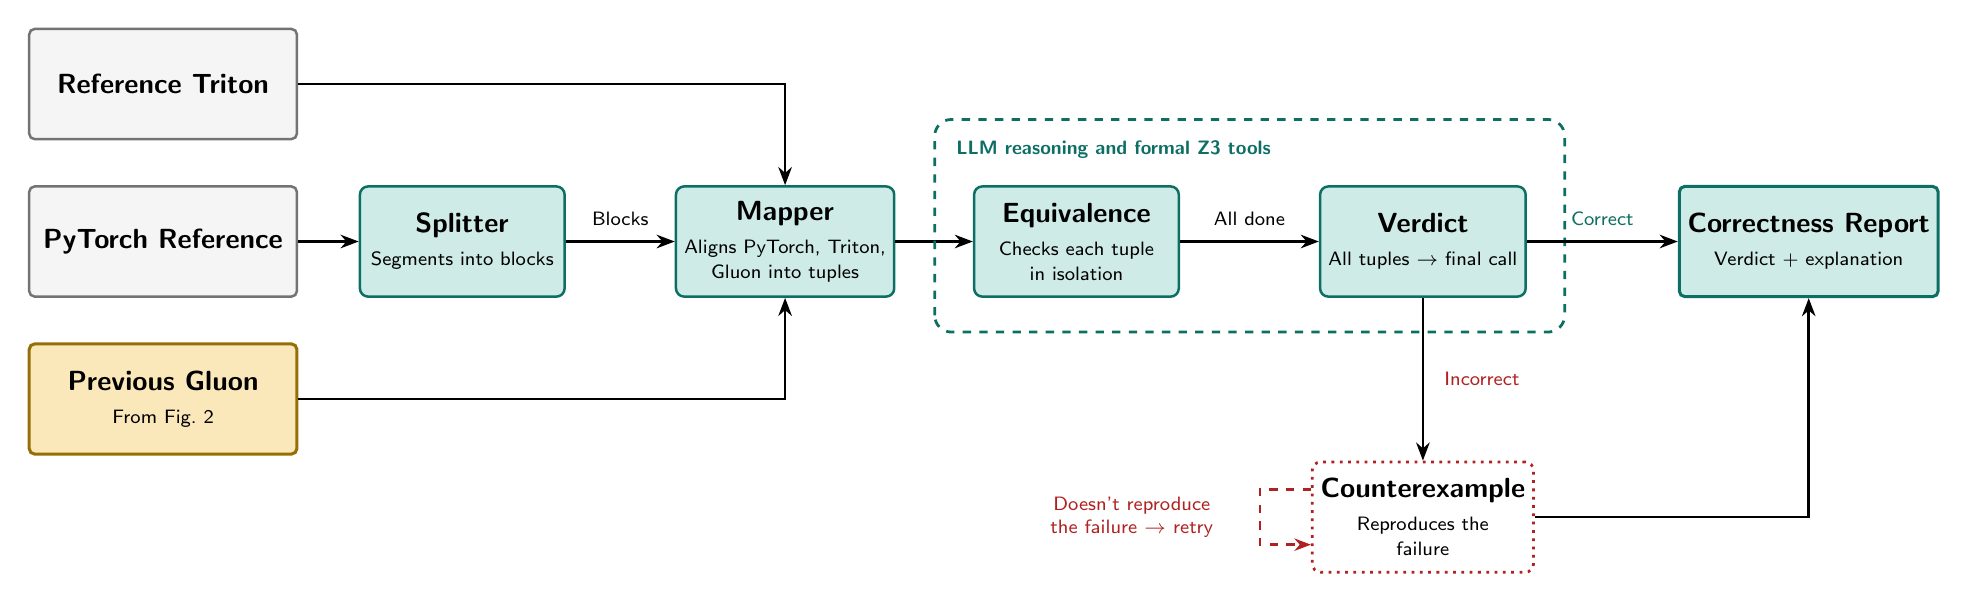
\begin{tikzpicture}[
  font=\sffamily,
  >=Stealth,
  titlestyle/.style={font=\sffamily\bfseries\Large},
  subtitlestyle/.style={font=\sffamily\itshape\small, text=black!55},
  boxsub/.style={font=\sffamily\scriptsize, align=center},
  tagstyle/.style={font=\sffamily\bfseries\scriptsize, text=corrteal},
  legendtext/.style={font=\sffamily\scriptsize},
  corrbox/.style={draw=corrteal, fill=corrtealfill, rounded corners=3pt, line width=0.9pt, minimum width=2.6cm, minimum height=1.4cm, align=center, inner sep=3pt, font=\sffamily\normalsize},
  srcartifact/.style={draw=black!55, fill=black!4, rounded corners=2pt, line width=0.9pt, align=center, minimum width=3.4cm, minimum height=1.4cm, inner sep=3pt, font=\sffamily\normalsize},
  gluonartifact/.style={draw=gluongold, fill=gluongoldfill, rounded corners=2pt, line width=1.1pt, align=center, minimum width=3.4cm, minimum height=1.4cm, inner sep=3pt, font=\sffamily\normalsize},
  reportartifact/.style={draw=corrteal, fill=corrtealfill, rounded corners=2pt, line width=1.1pt, align=center, minimum width=2.7cm, minimum height=1.4cm, inner sep=3pt, font=\sffamily\normalsize},
  counterbox/.style={draw=retryred, dotted, line width=1pt, rounded corners=3pt, fill=white, align=center, minimum width=2.6cm, minimum height=1.4cm, inner sep=3pt, font=\sffamily\normalsize},
  verifycontainer/.style={draw=corrteal, dashed, rounded corners=6pt, line width=1pt},
  mainarrow/.style={-{Stealth[length=2.3mm]}, line width=0.9pt, draw=black},
  retryarrow/.style={-{Stealth[length=2.1mm]}, line width=0.85pt, draw=retryred, dashed},
]

% ==================================================================
% Title band
% ==================================================================

% ==================================================================
% Step 1: Inputs (stacked -- all feed the checks below)
% ==================================================================
\node[srcartifact] (pytorch) at (0, 0) {\textbf{PyTorch Reference}};
\node[srcartifact] (reftriton) at (0, 2.0) {\textbf{Reference Triton}};
\node[gluonartifact] (prevgluon) at (0, -2.0) {\textbf{Previous Gluon}\\{\scriptsize From Fig.~2}};

% ==================================================================
% Step 2: Splitter -- Step 3: Mapper
% ==================================================================
\node[corrbox] (splitter) at (3.8, 0) {\textbf{Splitter}\\{\scriptsize Segments into blocks}};
\node[corrbox] (mapper) at (7.9, 0) {\textbf{Mapper}\\{\scriptsize Aligns PyTorch, Triton,}\\[-3pt]{\scriptsize Gluon into tuples}};

\draw[mainarrow] (pytorch.east) -- (splitter.west);
\draw[mainarrow] (splitter.east) -- (mapper.west)
  node[pos=0.5, above=2pt, boxsub] {\scriptsize Blocks};
\draw[mainarrow] (reftriton.east) -| (mapper.north);
\draw[mainarrow] (prevgluon.east) -| (mapper.south);

% ==================================================================
% Step 4: Equivalence + Verdict, wrapped in one verification container
% ==================================================================
\node[corrbox] (equiv) at (11.6, 0) {\textbf{Equivalence}\\{\scriptsize Checks each tuple}\\[-3pt]{\scriptsize in isolation}};
\draw[mainarrow] (mapper.east) -- (equiv.west);

\node[corrbox] (verdict) at (16.0, 0) {\textbf{Verdict}\\{\scriptsize All tuples $\to$ final call}};
\draw[mainarrow] (equiv.east) -- (verdict.west)
  node[pos=0.5, above=2pt, boxsub] {\scriptsize All done};

\draw[verifycontainer] (9.8,-1.15) rectangle (17.8,1.55);
\node[tagstyle, anchor=north west] at (9.95,1.4) {LLM reasoning and formal Z3 tools};

% ==================================================================
% Step 5: Counterexample (only reached on an incorrect verdict)
% ==================================================================
\node[counterbox] (counter) at (16.0, -3.5) {\textbf{Counterexample}\\{\scriptsize Reproduces the}\\[-3pt]{\scriptsize failure}};
\draw[mainarrow] (verdict.south) -- (counter.north)
  node[pos=0.5, right=4pt, boxsub, text=retryred] {\scriptsize Incorrect};

% ---- Retry: sharp-cornered square loop, well clear of the box edge ----
\coordinate (cLoopTop) at ($(counter.west)+(0,0.35)$);
\coordinate (cLoopBot) at ($(counter.west)+(0,-0.35)$);
\draw[retryarrow] (cLoopTop) -- ++(-0.65,0) -- ($(cLoopBot)+(-0.65,0)$) -- (cLoopBot);
\node[boxsub, text width=2.6cm, text=retryred, anchor=east] at ($(cLoopTop)+(-0.85,-0.35)$)
  {\scriptsize Doesn't reproduce the failure $\to$ retry};

% ==================================================================
% Step 6: Report -- receives the direct (correct) and counterexample paths
% ==================================================================
\node[reportartifact] (report) at (20.9, 0) {\textbf{Correctness Report}\\{\scriptsize Verdict + explanation}};
\draw[mainarrow] (verdict.east) -- (report.west)
  node[pos=0.5, above=2pt, boxsub, text=corrteal] {\scriptsize Correct};
\draw[mainarrow] (counter.east) -| (report.south);


\end{tikzpicture}
\end{document}
